
% Default to the notebook output style

    


% Inherit from the specified cell style.




    
\documentclass[11pt]{ctexart}

    
    
    \usepackage[T1]{fontenc}
    % Nicer default font (+ math font) than Computer Modern for most use cases
    \usepackage{mathpazo}

    % Basic figure setup, for now with no caption control since it's done
    % automatically by Pandoc (which extracts ![](path) syntax from Markdown).
    \usepackage{graphicx}
    % We will generate all images so they have a width \maxwidth. This means
    % that they will get their normal width if they fit onto the page, but
    % are scaled down if they would overflow the margins.
    \makeatletter
    \def\maxwidth{\ifdim\Gin@nat@width>\linewidth\linewidth
    \else\Gin@nat@width\fi}
    \makeatother
    \let\Oldincludegraphics\includegraphics
    % Set max figure width to be 80% of text width, for now hardcoded.
    \renewcommand{\includegraphics}[1]{\Oldincludegraphics[width=.8\maxwidth]{#1}}
    % Ensure that by default, figures have no caption (until we provide a
    % proper Figure object with a Caption API and a way to capture that
    % in the conversion process - todo).
    \usepackage{caption}
    \DeclareCaptionLabelFormat{nolabel}{}
    \captionsetup{labelformat=nolabel}

    \usepackage{adjustbox} % Used to constrain images to a maximum size 
    \usepackage{xcolor} % Allow colors to be defined
    \usepackage{enumerate} % Needed for markdown enumerations to work
    \usepackage{geometry} % Used to adjust the document margins
    \usepackage{amsmath} % Equations
    \usepackage{amssymb} % Equations
    \usepackage{textcomp} % defines textquotesingle
    % Hack from http://tex.stackexchange.com/a/47451/13684:
    \AtBeginDocument{%
        \def\PYZsq{\textquotesingle}% Upright quotes in Pygmentized code
    }
    \usepackage{upquote} % Upright quotes for verbatim code
    \usepackage{eurosym} % defines \euro
    \usepackage[mathletters]{ucs} % Extended unicode (utf-8) support
    \usepackage[utf8x]{inputenc} % Allow utf-8 characters in the tex document
    \usepackage{fancyvrb} % verbatim replacement that allows latex
    \usepackage{grffile} % extends the file name processing of package graphics 
                         % to support a larger range 
    % The hyperref package gives us a pdf with properly built
    % internal navigation ('pdf bookmarks' for the table of contents,
    % internal cross-reference links, web links for URLs, etc.)
    \usepackage{hyperref}
    \usepackage{longtable} % longtable support required by pandoc >1.10
    \usepackage{booktabs}  % table support for pandoc > 1.12.2
    \usepackage[inline]{enumitem} % IRkernel/repr support (it uses the enumerate* environment)
    \usepackage[normalem]{ulem} % ulem is needed to support strikethroughs (\sout)
                                % normalem makes italics be italics, not underlines
    \usepackage{mathrsfs}
    

    
    
    % Colors for the hyperref package
    \definecolor{urlcolor}{rgb}{0,.145,.698}
    \definecolor{linkcolor}{rgb}{.71,0.21,0.01}
    \definecolor{citecolor}{rgb}{.12,.54,.11}

    % ANSI colors
    \definecolor{ansi-black}{HTML}{3E424D}
    \definecolor{ansi-black-intense}{HTML}{282C36}
    \definecolor{ansi-red}{HTML}{E75C58}
    \definecolor{ansi-red-intense}{HTML}{B22B31}
    \definecolor{ansi-green}{HTML}{00A250}
    \definecolor{ansi-green-intense}{HTML}{007427}
    \definecolor{ansi-yellow}{HTML}{DDB62B}
    \definecolor{ansi-yellow-intense}{HTML}{B27D12}
    \definecolor{ansi-blue}{HTML}{208FFB}
    \definecolor{ansi-blue-intense}{HTML}{0065CA}
    \definecolor{ansi-magenta}{HTML}{D160C4}
    \definecolor{ansi-magenta-intense}{HTML}{A03196}
    \definecolor{ansi-cyan}{HTML}{60C6C8}
    \definecolor{ansi-cyan-intense}{HTML}{258F8F}
    \definecolor{ansi-white}{HTML}{C5C1B4}
    \definecolor{ansi-white-intense}{HTML}{A1A6B2}
    \definecolor{ansi-default-inverse-fg}{HTML}{FFFFFF}
    \definecolor{ansi-default-inverse-bg}{HTML}{000000}

    % commands and environments needed by pandoc snippets
    % extracted from the output of `pandoc -s`
    \providecommand{\tightlist}{%
      \setlength{\itemsep}{0pt}\setlength{\parskip}{0pt}}
    \DefineVerbatimEnvironment{Highlighting}{Verbatim}{commandchars=\\\{\}}
    % Add ',fontsize=\small' for more characters per line
    \newenvironment{Shaded}{}{}
    \newcommand{\KeywordTok}[1]{\textcolor[rgb]{0.00,0.44,0.13}{\textbf{{#1}}}}
    \newcommand{\DataTypeTok}[1]{\textcolor[rgb]{0.56,0.13,0.00}{{#1}}}
    \newcommand{\DecValTok}[1]{\textcolor[rgb]{0.25,0.63,0.44}{{#1}}}
    \newcommand{\BaseNTok}[1]{\textcolor[rgb]{0.25,0.63,0.44}{{#1}}}
    \newcommand{\FloatTok}[1]{\textcolor[rgb]{0.25,0.63,0.44}{{#1}}}
    \newcommand{\CharTok}[1]{\textcolor[rgb]{0.25,0.44,0.63}{{#1}}}
    \newcommand{\StringTok}[1]{\textcolor[rgb]{0.25,0.44,0.63}{{#1}}}
    \newcommand{\CommentTok}[1]{\textcolor[rgb]{0.38,0.63,0.69}{\textit{{#1}}}}
    \newcommand{\OtherTok}[1]{\textcolor[rgb]{0.00,0.44,0.13}{{#1}}}
    \newcommand{\AlertTok}[1]{\textcolor[rgb]{1.00,0.00,0.00}{\textbf{{#1}}}}
    \newcommand{\FunctionTok}[1]{\textcolor[rgb]{0.02,0.16,0.49}{{#1}}}
    \newcommand{\RegionMarkerTok}[1]{{#1}}
    \newcommand{\ErrorTok}[1]{\textcolor[rgb]{1.00,0.00,0.00}{\textbf{{#1}}}}
    \newcommand{\NormalTok}[1]{{#1}}
    
    % Additional commands for more recent versions of Pandoc
    \newcommand{\ConstantTok}[1]{\textcolor[rgb]{0.53,0.00,0.00}{{#1}}}
    \newcommand{\SpecialCharTok}[1]{\textcolor[rgb]{0.25,0.44,0.63}{{#1}}}
    \newcommand{\VerbatimStringTok}[1]{\textcolor[rgb]{0.25,0.44,0.63}{{#1}}}
    \newcommand{\SpecialStringTok}[1]{\textcolor[rgb]{0.73,0.40,0.53}{{#1}}}
    \newcommand{\ImportTok}[1]{{#1}}
    \newcommand{\DocumentationTok}[1]{\textcolor[rgb]{0.73,0.13,0.13}{\textit{{#1}}}}
    \newcommand{\AnnotationTok}[1]{\textcolor[rgb]{0.38,0.63,0.69}{\textbf{\textit{{#1}}}}}
    \newcommand{\CommentVarTok}[1]{\textcolor[rgb]{0.38,0.63,0.69}{\textbf{\textit{{#1}}}}}
    \newcommand{\VariableTok}[1]{\textcolor[rgb]{0.10,0.09,0.49}{{#1}}}
    \newcommand{\ControlFlowTok}[1]{\textcolor[rgb]{0.00,0.44,0.13}{\textbf{{#1}}}}
    \newcommand{\OperatorTok}[1]{\textcolor[rgb]{0.40,0.40,0.40}{{#1}}}
    \newcommand{\BuiltInTok}[1]{{#1}}
    \newcommand{\ExtensionTok}[1]{{#1}}
    \newcommand{\PreprocessorTok}[1]{\textcolor[rgb]{0.74,0.48,0.00}{{#1}}}
    \newcommand{\AttributeTok}[1]{\textcolor[rgb]{0.49,0.56,0.16}{{#1}}}
    \newcommand{\InformationTok}[1]{\textcolor[rgb]{0.38,0.63,0.69}{\textbf{\textit{{#1}}}}}
    \newcommand{\WarningTok}[1]{\textcolor[rgb]{0.38,0.63,0.69}{\textbf{\textit{{#1}}}}}
    
    
    % Define a nice break command that doesn't care if a line doesn't already
    % exist.
    \def\br{\hspace*{\fill} \\* }
    % Math Jax compatibility definitions
    \def\gt{>}
    \def\lt{<}
    \let\Oldtex\TeX
    \let\Oldlatex\LaTeX
    \renewcommand{\TeX}{\textrm{\Oldtex}}
    \renewcommand{\LaTeX}{\textrm{\Oldlatex}}
    % Document parameters
    % Document title
    \title{\textbf{\LARGE{PowerShell学习笔记}}}
    \author{Cheng Jun}
    \date{\today}
    
    
\usepackage{xeCJK}
\setCJKmainfont{思源宋体 CN}[BoldFont = 思源宋体 CN Bold]
\setCJKsansfont{思源黑体 CN}
\setmainfont{思源宋体 CN}[BoldFont = 思源宋体 CN Bold]
\setsansfont{思源黑体 CN}
\setmonofont{Source Code Pro}

\hypersetup{
    breaklinks=true,  % so long urls are correctly broken across lines
    colorlinks=true,
    urlcolor=urlcolor,
    linkcolor=linkcolor,
    citecolor=citecolor,
    pdfauthor={Cheng Jun},
          pdftitle={PowerShell学习笔记},
          pdfsubject={PowerShell},
          pdfkeywords={PowerShell,脚本},
          pdfproducer={LaTeX},
          pdfcreator={XeLaTeX}
}
    
    
    
    
    

    % Pygments definitions
    
\makeatletter
\def\PY@reset{\let\PY@it=\relax \let\PY@bf=\relax%
    \let\PY@ul=\relax \let\PY@tc=\relax%
    \let\PY@bc=\relax \let\PY@ff=\relax}
\def\PY@tok#1{\csname PY@tok@#1\endcsname}
\def\PY@toks#1+{\ifx\relax#1\empty\else%
    \PY@tok{#1}\expandafter\PY@toks\fi}
\def\PY@do#1{\PY@bc{\PY@tc{\PY@ul{%
    \PY@it{\PY@bf{\PY@ff{#1}}}}}}}
\def\PY#1#2{\PY@reset\PY@toks#1+\relax+\PY@do{#2}}

\expandafter\def\csname PY@tok@w\endcsname{\def\PY@tc##1{\textcolor[rgb]{0.73,0.73,0.73}{##1}}}
\expandafter\def\csname PY@tok@c\endcsname{\let\PY@it=\textit\def\PY@tc##1{\textcolor[rgb]{0.25,0.50,0.50}{##1}}}
\expandafter\def\csname PY@tok@cp\endcsname{\def\PY@tc##1{\textcolor[rgb]{0.74,0.48,0.00}{##1}}}
\expandafter\def\csname PY@tok@k\endcsname{\let\PY@bf=\textbf\def\PY@tc##1{\textcolor[rgb]{0.00,0.50,0.00}{##1}}}
\expandafter\def\csname PY@tok@kp\endcsname{\def\PY@tc##1{\textcolor[rgb]{0.00,0.50,0.00}{##1}}}
\expandafter\def\csname PY@tok@kt\endcsname{\def\PY@tc##1{\textcolor[rgb]{0.69,0.00,0.25}{##1}}}
\expandafter\def\csname PY@tok@o\endcsname{\def\PY@tc##1{\textcolor[rgb]{0.40,0.40,0.40}{##1}}}
\expandafter\def\csname PY@tok@ow\endcsname{\let\PY@bf=\textbf\def\PY@tc##1{\textcolor[rgb]{0.67,0.13,1.00}{##1}}}
\expandafter\def\csname PY@tok@nb\endcsname{\def\PY@tc##1{\textcolor[rgb]{0.00,0.50,0.00}{##1}}}
\expandafter\def\csname PY@tok@nf\endcsname{\def\PY@tc##1{\textcolor[rgb]{0.00,0.00,1.00}{##1}}}
\expandafter\def\csname PY@tok@nc\endcsname{\let\PY@bf=\textbf\def\PY@tc##1{\textcolor[rgb]{0.00,0.00,1.00}{##1}}}
\expandafter\def\csname PY@tok@nn\endcsname{\let\PY@bf=\textbf\def\PY@tc##1{\textcolor[rgb]{0.00,0.00,1.00}{##1}}}
\expandafter\def\csname PY@tok@ne\endcsname{\let\PY@bf=\textbf\def\PY@tc##1{\textcolor[rgb]{0.82,0.25,0.23}{##1}}}
\expandafter\def\csname PY@tok@nv\endcsname{\def\PY@tc##1{\textcolor[rgb]{0.10,0.09,0.49}{##1}}}
\expandafter\def\csname PY@tok@no\endcsname{\def\PY@tc##1{\textcolor[rgb]{0.53,0.00,0.00}{##1}}}
\expandafter\def\csname PY@tok@nl\endcsname{\def\PY@tc##1{\textcolor[rgb]{0.63,0.63,0.00}{##1}}}
\expandafter\def\csname PY@tok@ni\endcsname{\let\PY@bf=\textbf\def\PY@tc##1{\textcolor[rgb]{0.60,0.60,0.60}{##1}}}
\expandafter\def\csname PY@tok@na\endcsname{\def\PY@tc##1{\textcolor[rgb]{0.49,0.56,0.16}{##1}}}
\expandafter\def\csname PY@tok@nt\endcsname{\let\PY@bf=\textbf\def\PY@tc##1{\textcolor[rgb]{0.00,0.50,0.00}{##1}}}
\expandafter\def\csname PY@tok@nd\endcsname{\def\PY@tc##1{\textcolor[rgb]{0.67,0.13,1.00}{##1}}}
\expandafter\def\csname PY@tok@s\endcsname{\def\PY@tc##1{\textcolor[rgb]{0.73,0.13,0.13}{##1}}}
\expandafter\def\csname PY@tok@sd\endcsname{\let\PY@it=\textit\def\PY@tc##1{\textcolor[rgb]{0.73,0.13,0.13}{##1}}}
\expandafter\def\csname PY@tok@si\endcsname{\let\PY@bf=\textbf\def\PY@tc##1{\textcolor[rgb]{0.73,0.40,0.53}{##1}}}
\expandafter\def\csname PY@tok@se\endcsname{\let\PY@bf=\textbf\def\PY@tc##1{\textcolor[rgb]{0.73,0.40,0.13}{##1}}}
\expandafter\def\csname PY@tok@sr\endcsname{\def\PY@tc##1{\textcolor[rgb]{0.73,0.40,0.53}{##1}}}
\expandafter\def\csname PY@tok@ss\endcsname{\def\PY@tc##1{\textcolor[rgb]{0.10,0.09,0.49}{##1}}}
\expandafter\def\csname PY@tok@sx\endcsname{\def\PY@tc##1{\textcolor[rgb]{0.00,0.50,0.00}{##1}}}
\expandafter\def\csname PY@tok@m\endcsname{\def\PY@tc##1{\textcolor[rgb]{0.40,0.40,0.40}{##1}}}
\expandafter\def\csname PY@tok@gh\endcsname{\let\PY@bf=\textbf\def\PY@tc##1{\textcolor[rgb]{0.00,0.00,0.50}{##1}}}
\expandafter\def\csname PY@tok@gu\endcsname{\let\PY@bf=\textbf\def\PY@tc##1{\textcolor[rgb]{0.50,0.00,0.50}{##1}}}
\expandafter\def\csname PY@tok@gd\endcsname{\def\PY@tc##1{\textcolor[rgb]{0.63,0.00,0.00}{##1}}}
\expandafter\def\csname PY@tok@gi\endcsname{\def\PY@tc##1{\textcolor[rgb]{0.00,0.63,0.00}{##1}}}
\expandafter\def\csname PY@tok@gr\endcsname{\def\PY@tc##1{\textcolor[rgb]{1.00,0.00,0.00}{##1}}}
\expandafter\def\csname PY@tok@ge\endcsname{\let\PY@it=\textit}
\expandafter\def\csname PY@tok@gs\endcsname{\let\PY@bf=\textbf}
\expandafter\def\csname PY@tok@gp\endcsname{\let\PY@bf=\textbf\def\PY@tc##1{\textcolor[rgb]{0.00,0.00,0.50}{##1}}}
\expandafter\def\csname PY@tok@go\endcsname{\def\PY@tc##1{\textcolor[rgb]{0.53,0.53,0.53}{##1}}}
\expandafter\def\csname PY@tok@gt\endcsname{\def\PY@tc##1{\textcolor[rgb]{0.00,0.27,0.87}{##1}}}
\expandafter\def\csname PY@tok@err\endcsname{\def\PY@bc##1{\setlength{\fboxsep}{0pt}\fcolorbox[rgb]{1.00,0.00,0.00}{1,1,1}{\strut ##1}}}
\expandafter\def\csname PY@tok@kc\endcsname{\let\PY@bf=\textbf\def\PY@tc##1{\textcolor[rgb]{0.00,0.50,0.00}{##1}}}
\expandafter\def\csname PY@tok@kd\endcsname{\let\PY@bf=\textbf\def\PY@tc##1{\textcolor[rgb]{0.00,0.50,0.00}{##1}}}
\expandafter\def\csname PY@tok@kn\endcsname{\let\PY@bf=\textbf\def\PY@tc##1{\textcolor[rgb]{0.00,0.50,0.00}{##1}}}
\expandafter\def\csname PY@tok@kr\endcsname{\let\PY@bf=\textbf\def\PY@tc##1{\textcolor[rgb]{0.00,0.50,0.00}{##1}}}
\expandafter\def\csname PY@tok@bp\endcsname{\def\PY@tc##1{\textcolor[rgb]{0.00,0.50,0.00}{##1}}}
\expandafter\def\csname PY@tok@fm\endcsname{\def\PY@tc##1{\textcolor[rgb]{0.00,0.00,1.00}{##1}}}
\expandafter\def\csname PY@tok@vc\endcsname{\def\PY@tc##1{\textcolor[rgb]{0.10,0.09,0.49}{##1}}}
\expandafter\def\csname PY@tok@vg\endcsname{\def\PY@tc##1{\textcolor[rgb]{0.10,0.09,0.49}{##1}}}
\expandafter\def\csname PY@tok@vi\endcsname{\def\PY@tc##1{\textcolor[rgb]{0.10,0.09,0.49}{##1}}}
\expandafter\def\csname PY@tok@vm\endcsname{\def\PY@tc##1{\textcolor[rgb]{0.10,0.09,0.49}{##1}}}
\expandafter\def\csname PY@tok@sa\endcsname{\def\PY@tc##1{\textcolor[rgb]{0.73,0.13,0.13}{##1}}}
\expandafter\def\csname PY@tok@sb\endcsname{\def\PY@tc##1{\textcolor[rgb]{0.73,0.13,0.13}{##1}}}
\expandafter\def\csname PY@tok@sc\endcsname{\def\PY@tc##1{\textcolor[rgb]{0.73,0.13,0.13}{##1}}}
\expandafter\def\csname PY@tok@dl\endcsname{\def\PY@tc##1{\textcolor[rgb]{0.73,0.13,0.13}{##1}}}
\expandafter\def\csname PY@tok@s2\endcsname{\def\PY@tc##1{\textcolor[rgb]{0.73,0.13,0.13}{##1}}}
\expandafter\def\csname PY@tok@sh\endcsname{\def\PY@tc##1{\textcolor[rgb]{0.73,0.13,0.13}{##1}}}
\expandafter\def\csname PY@tok@s1\endcsname{\def\PY@tc##1{\textcolor[rgb]{0.73,0.13,0.13}{##1}}}
\expandafter\def\csname PY@tok@mb\endcsname{\def\PY@tc##1{\textcolor[rgb]{0.40,0.40,0.40}{##1}}}
\expandafter\def\csname PY@tok@mf\endcsname{\def\PY@tc##1{\textcolor[rgb]{0.40,0.40,0.40}{##1}}}
\expandafter\def\csname PY@tok@mh\endcsname{\def\PY@tc##1{\textcolor[rgb]{0.40,0.40,0.40}{##1}}}
\expandafter\def\csname PY@tok@mi\endcsname{\def\PY@tc##1{\textcolor[rgb]{0.40,0.40,0.40}{##1}}}
\expandafter\def\csname PY@tok@il\endcsname{\def\PY@tc##1{\textcolor[rgb]{0.40,0.40,0.40}{##1}}}
\expandafter\def\csname PY@tok@mo\endcsname{\def\PY@tc##1{\textcolor[rgb]{0.40,0.40,0.40}{##1}}}
\expandafter\def\csname PY@tok@ch\endcsname{\let\PY@it=\textit\def\PY@tc##1{\textcolor[rgb]{0.25,0.50,0.50}{##1}}}
\expandafter\def\csname PY@tok@cm\endcsname{\let\PY@it=\textit\def\PY@tc##1{\textcolor[rgb]{0.25,0.50,0.50}{##1}}}
\expandafter\def\csname PY@tok@cpf\endcsname{\let\PY@it=\textit\def\PY@tc##1{\textcolor[rgb]{0.25,0.50,0.50}{##1}}}
\expandafter\def\csname PY@tok@c1\endcsname{\let\PY@it=\textit\def\PY@tc##1{\textcolor[rgb]{0.25,0.50,0.50}{##1}}}
\expandafter\def\csname PY@tok@cs\endcsname{\let\PY@it=\textit\def\PY@tc##1{\textcolor[rgb]{0.25,0.50,0.50}{##1}}}

\def\PYZbs{\char`\\}
\def\PYZus{\char`\_}
\def\PYZob{\char`\{}
\def\PYZcb{\char`\}}
\def\PYZca{\char`\^}
\def\PYZam{\char`\&}
\def\PYZlt{\char`\<}
\def\PYZgt{\char`\>}
\def\PYZsh{\char`\#}
\def\PYZpc{\char`\%}
\def\PYZdl{\char`\$}
\def\PYZhy{\char`\-}
\def\PYZsq{\char`\'}
\def\PYZdq{\char`\"}
\def\PYZti{\char`\~}
% for compatibility with earlier versions
\def\PYZat{@}
\def\PYZlb{[}
\def\PYZrb{]}
\makeatother


    % Exact colors from NB
    \definecolor{incolor}{rgb}{0.0, 0.0, 0.5}
    \definecolor{outcolor}{rgb}{0.545, 0.0, 0.0}



    
    % Prevent overflowing lines due to hard-to-break entities
    \sloppy 
    % Setup hyperref package
    \hypersetup{
      breaklinks=true,  % so long urls are correctly broken across lines
      colorlinks=true,
      urlcolor=urlcolor,
      linkcolor=linkcolor,
      citecolor=citecolor,
      }
    % Slightly bigger margins than the latex defaults
    
    \geometry{verbose,tmargin=1in,bmargin=1in,lmargin=1in,rmargin=1in}
    
    

    \begin{document}
    
    
    \maketitle
    \tableofcontents
    \clearpage
    
    

    
    \hypertarget{ux524dux8a00}{%
\section{前言}\label{ux524dux8a00}}

    \hypertarget{ux7b14ux8bb0ux4f5cux8005}{%
\subsection{笔记作者}\label{ux7b14ux8bb0ux4f5cux8005}}

    实证研究小青年。

日常研究和关注经济、金融与会计等领域的问题,主要采用计量经济学和其他数据分析手法撰写学术论
文和研究报告。

研究之余,泛读文史哲,关注自由与开源动态。在日常研究和工作中,喜欢使用最新的软件工具,并且喜欢选用自由和开源工具。

邮箱:cheng081@qq.com

Github:https://github.com/chengjun90

欢迎交流。

    \hypertarget{ux5b66ux4e60ux76eeux7684}{%
\subsection{学习目的}\label{ux5b66ux4e60ux76eeux7684}}

    不是完整的掌握PowerShell,而是了解基本的PowerShell的应用,方便在研究工作和生活中需要的时候用一点脚本。

比如:

\begin{itemize}
\tightlist
\item
  \emph{Data Science at the Command Line}
\item
  Command Line Tricks For Data Scientists
\end{itemize}

    \hypertarget{ux51c6ux5907ux5de5ux4f5c}{%
\subsection{准备工作}\label{ux51c6ux5907ux5de5ux4f5c}}

    \hypertarget{ux5b89ux88c5pythonjupyter-lab}{%
\subsubsection{安装Python+Jupyter
Lab}\label{ux5b89ux88c5pythonjupyter-lab}}

这个就不说了,很好安装。直接搜索。

    \hypertarget{ux5b89ux88c5powershell-kernel}{%
\subsubsection{安装PowerShell
Kernel}\label{ux5b89ux88c5powershell-kernel}}

可以使用这里https://github.com/vors/jupyter-powershell提供的包。

\begin{Shaded}
\begin{Highlighting}[]
\NormalTok{pip install powershell_kernel}
\NormalTok{python }\OperatorTok{-}\NormalTok{m powershell_kernel.install}
\end{Highlighting}
\end{Shaded}

这样就可以在Jupyter Lab中学习和使用Powershell了。

    \hypertarget{ux5b66ux4e60ux73afux5883}{%
\subsection{学习环境}\label{ux5b66ux4e60ux73afux5883}}

    \hypertarget{ux7cfbux7edfux81eaux5e26ux7684powershell}{%
\subsubsection{系统自带的Powershell}\label{ux7cfbux7edfux81eaux5e26ux7684powershell}}

这里是Powershell版本是5.1。

    \begin{Verbatim}[commandchars=\\\{\}]
{\color{incolor}In [{\color{incolor}1}]:} \PY{n+nv}{\PYZdl{}psversiontable}
\end{Verbatim}

    \begin{Verbatim}[commandchars=\\\{\}]

Name                           Value                                                                                   
----                           -----                                                                                   
PSVersion                      5.1.17134.228                                                                           
PSEdition                      Desktop                                                                                 
PSCompatibleVersions           \{1.0, 2.0, 3.0, 4.0{\ldots}\}                                                                 
BuildVersion                   10.0.17134.228                                                                          
CLRVersion                     4.0.30319.42000                                                                         
WSManStackVersion              3.0                                                                                     
PSRemotingProtocolVersion      2.3                                                                                     
SerializationVersion           1.1.0.1                                                                                 



    \end{Verbatim}

    \hypertarget{powershell-core}{%
\subsubsection{Powershell Core}\label{powershell-core}}

当然也可以自行安装跨平台的\href{https://github.com/PowerShell/PowerShell/releases}{Powershell
Core}。

\begin{Shaded}
\begin{Highlighting}[]
\FunctionTok{PS}\NormalTok{ C:\textbackslash{}Users\textbackslash{}Cheng> }\VariableTok{$psversiontable}

\NormalTok{Name                           Value}
\NormalTok{----                           -----}
\NormalTok{PSVersion                      6.}\FunctionTok{1}\NormalTok{.}\FunctionTok{0}
\NormalTok{PSEdition                      Core}
\NormalTok{GitCommitId                    6.}\FunctionTok{1}\NormalTok{.}\FunctionTok{0}
\NormalTok{OS                             Microsoft Windows 10.}\FunctionTok{0}\NormalTok{.}\FunctionTok{17134}
\NormalTok{Platform                       Win32NT}
\NormalTok{PSCompatibleVersions           \{1.}\FunctionTok{0}\NormalTok{, 2.}\FunctionTok{0}\NormalTok{, 3.}\FunctionTok{0}\NormalTok{, 4.}\FunctionTok{0}\NormalTok{...\}}
\NormalTok{PSRemotingProtocolVersion      2.}\FunctionTok{3}
\NormalTok{SerializationVersion           1.}\FunctionTok{1}\NormalTok{.}\FunctionTok{0}\NormalTok{.}\FunctionTok{1}
\NormalTok{WSManStackVersion              3.}\FunctionTok{0}

\end{Highlighting}

\end{Shaded}

2018年,Powershell
Core已经支持utf-8编码了,可以使用第三方字体,例如\href{https://github.com/adobe-fonts/source-code-pro}{Source
Code Pro}。

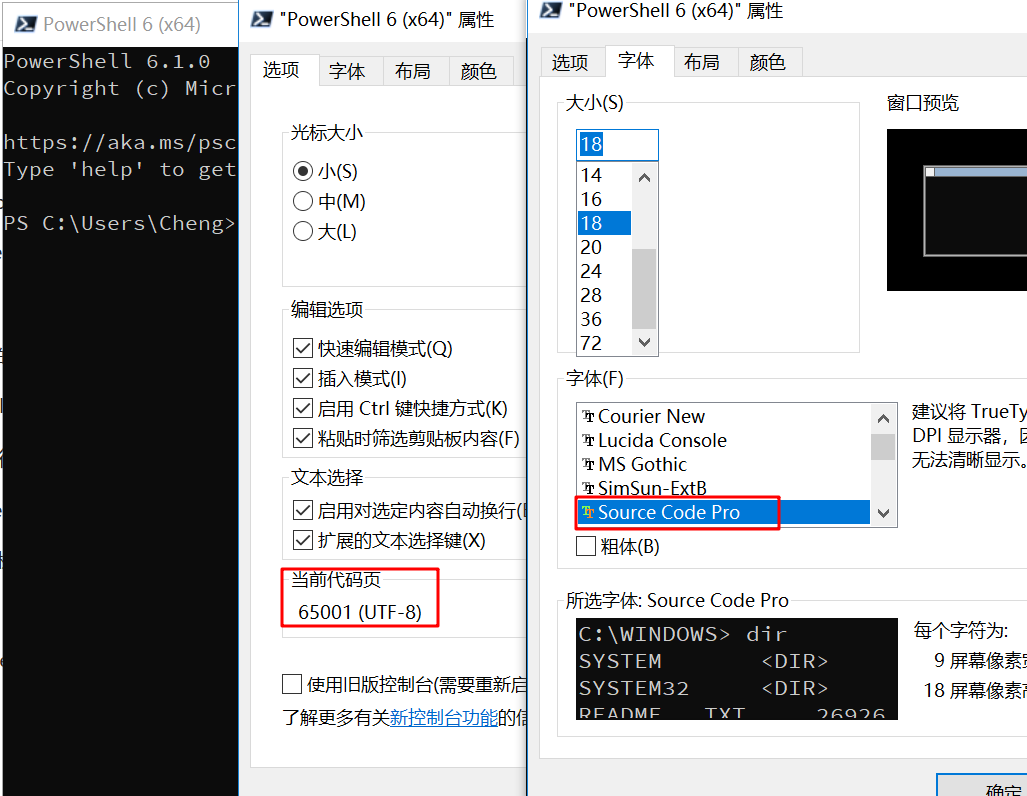
\includegraphics{image/ps5-core.png}

    \hypertarget{ux7f16ux8f91ux548cux8fd0ux884cux547dux4ee4}{%
\subsection{编辑和运行命令}\label{ux7f16ux8f91ux548cux8fd0ux884cux547dux4ee4}}

    \hypertarget{ux542fux52a8powershell}{%
\subsubsection{启动Powershell}\label{ux542fux52a8powershell}}

直接在窗口输入``Powershell'',然后点击。

如果是想调用Powershell Core,那么就输入``pwsh''。

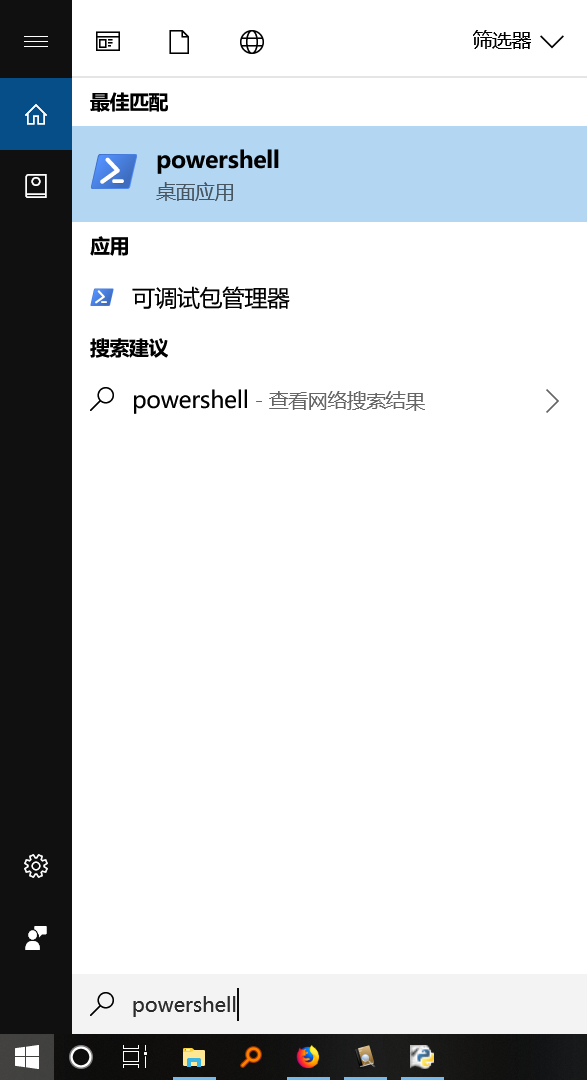
\includegraphics{image/ps1.png}

    \hypertarget{ux4ee5ux7ba1ux7406ux8005ux6743ux9650ux6a21ux5f0fux542fux52a8powershell}{%
\subsubsection{以管理者权限模式启动Powershell}\label{ux4ee5ux7ba1ux7406ux8005ux6743ux9650ux6a21ux5f0fux542fux52a8powershell}}

例如在按照Python包的时候,常常需要进入这种模式。

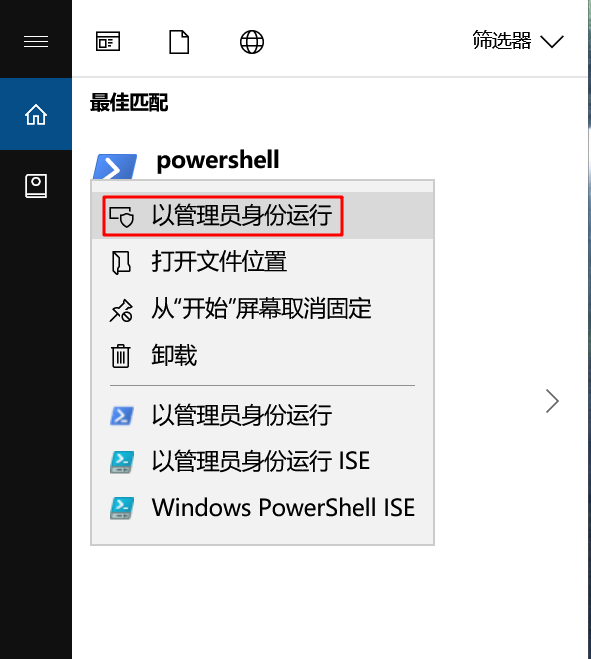
\includegraphics{image/ps2-ad.png}

    \hypertarget{ux8f93ux5165ux547dux4ee4}{%
\subsubsection{输入命令}\label{ux8f93ux5165ux547dux4ee4}}

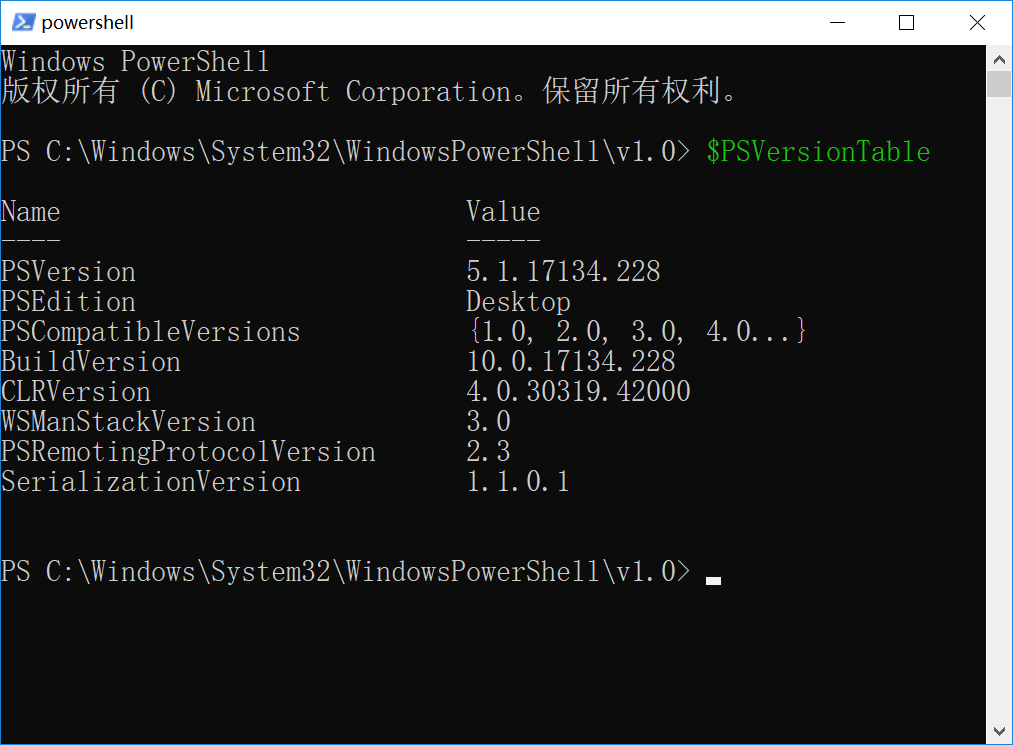
\includegraphics{image/ps3-code.png}

    \hypertarget{ux5728vs-codeux4e2dux7f16ux8f91ux548cux8fd0ux884cux547dux4ee4}{%
\subsubsection{在VS
Code中编辑和运行命令}\label{ux5728vs-codeux4e2dux7f16ux8f91ux548cux8fd0ux884cux547dux4ee4}}

Powershell文件的类型名称是ps1。

点击1或者2来运行Powershell命令。

    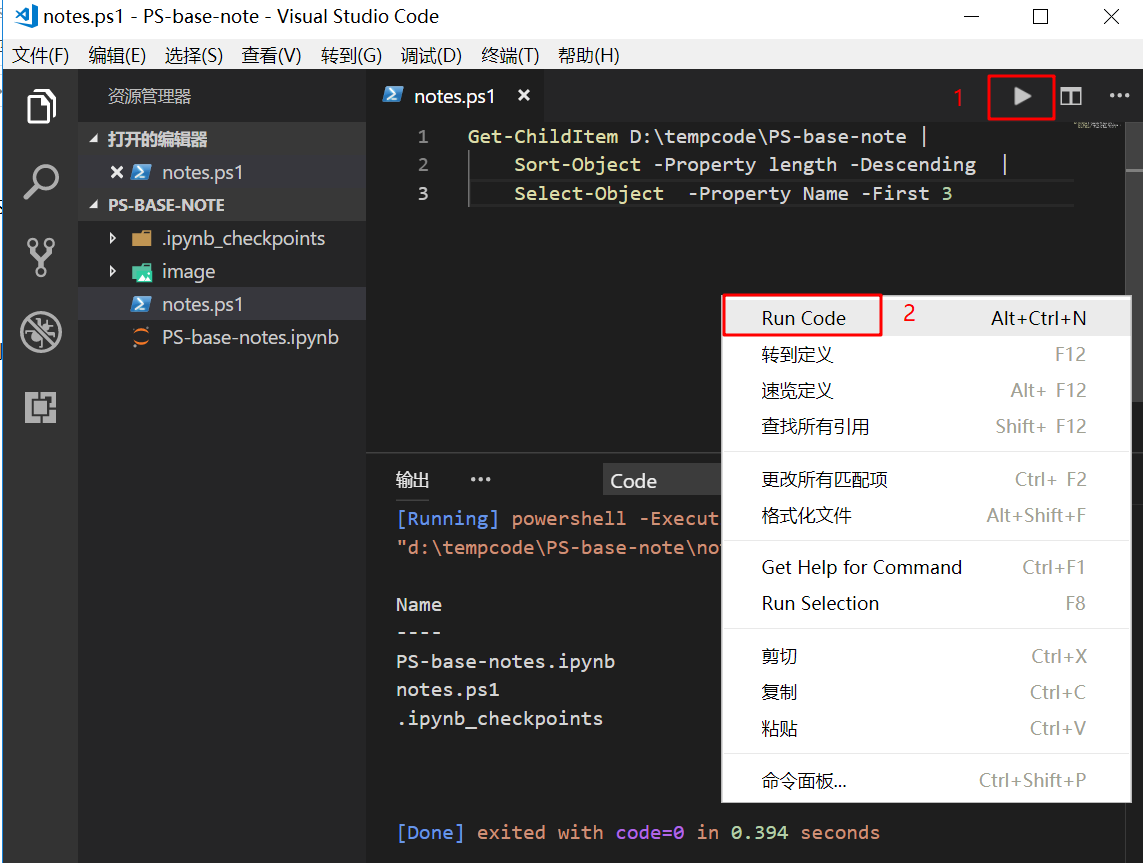
\includegraphics{image/ps4-run.png}

    \hypertarget{ux53c2ux8003ux6750ux6599}{%
\subsection{参考材料}\label{ux53c2ux8003ux6750ux6599}}

\begin{itemize}
\tightlist
\item
  \href{https://docs.microsoft.com/zh-cn/powershell/scripting/powershell-scripting?view=powershell-6}{微软PowerShell材料}
\item
  \emph{Learn Windows PowerShell in a Month of Lunches}
\end{itemize}

    \hypertarget{ux57faux7840}{%
\section{基础}\label{ux57faux7840}}

    \hypertarget{ux5e2eux52a9}{%
\subsection{帮助}\label{ux5e2eux52a9}}

善于使用Get-Help命令来查找帮助文件

    \begin{Verbatim}[commandchars=\\\{\}]
{\color{incolor}In [{\color{incolor}2}]:} \PY{n+nb}{Get\PYZhy{}Help} \PY{n+nb}{Get\PYZhy{}ChildItem}
\end{Verbatim}

    \begin{Verbatim}[commandchars=\\\{\}]

■■■    Get-ChildItem
    
■■■
    Get-ChildItem [[-Path] <string[]>] [[-Filter] <string>]  [<CommonParameters>]
    
    Get-ChildItem [[-Filter] <string>]  [<CommonParameters>]
    

■■■
    gci
    ls
    dir
    

■■ע
    Get-Help ■■˼■■■■■■■■■■cmdlet ■İ■■■■■■■■■■■ʾ■■■ְ■■■■
        -- ■Ҫ■■■■■■װ■■■■■■cmdlet ■■■■■■■■■■■■■■ʹ■ Update-Help■■
        -- ■Ҫ■■■■■鿴■■cmdlet ■İ■■■■■■■■■■: "Get-Help Get-ChildItem -Online" ■■
           ת■■ https://go.microsoft.com/fwlink/?LinkID=113308■■




    \end{Verbatim}

    有的时候命令记不全,那么可以使用Tab键来补全命令。

或者使用Show-Command命令来帮助自己。Show-Command可以弹出窗口来选择命令、填写命令参数。

    \hypertarget{ux522bux540d}{%
\subsection{别名}\label{ux522bux540d}}

Powershell的命令很多有别名,可以理解成命令的简短昵称,便于输入命令。

    \begin{Verbatim}[commandchars=\\\{\}]
{\color{incolor}In [{\color{incolor}3}]:} \PY{n+nb}{Get\PYZhy{}Alias} \PY{n}{\PYZhy{}Definition} \PY{l+s+s2}{\PYZdq{}}\PY{l+s+s2}{Set\PYZhy{}Location}\PY{l+s+s2}{\PYZdq{}}
\end{Verbatim}

    \begin{Verbatim}[commandchars=\\\{\}]

CommandType     Name                                               Version    Source                                   
-----------     ----                                               -------    ------                                   
Alias           cd -> Set-Location                                                                                     
Alias           chdir -> Set-Location                                                                                  
Alias           sl -> Set-Location                                                                                     



    \end{Verbatim}

    \begin{Verbatim}[commandchars=\\\{\}]
{\color{incolor}In [{\color{incolor}4}]:} \PY{n+nb}{Get\PYZhy{}Alias} \PY{n}{\PYZhy{}Definition} \PY{l+s+s2}{\PYZdq{}}\PY{l+s+s2}{Get\PYZhy{}ChildItem}\PY{l+s+s2}{\PYZdq{}}
\end{Verbatim}

    \begin{Verbatim}[commandchars=\\\{\}]

CommandType     Name                                               Version    Source                                   
-----------     ----                                               -------    ------                                   
Alias           dir -> Get-ChildItem                                                                                   
Alias           gci -> Get-ChildItem                                                                                   
Alias           ls -> Get-ChildItem                                                                                    



    \end{Verbatim}

    \hypertarget{ux6e05ux7406ux5c4fux5e55}{%
\subsection{清理屏幕}\label{ux6e05ux7406ux5c4fux5e55}}

直接使用cls命令即可。

    \hypertarget{ux6587ux4ef6ux64cdux4f5c}{%
\section{文件操作}\label{ux6587ux4ef6ux64cdux4f5c}}

    \hypertarget{ux8bbeux7f6eux8defux5f84}{%
\subsection{设置路径}\label{ux8bbeux7f6eux8defux5f84}}

比如我们常常需要切换工作路径。这个时候需要使用Set-Location命令。

不过我常常使用其别名cd。

\begin{Shaded}
\begin{Highlighting}[]
\FunctionTok{cd}\NormalTok{ D:\textbackslash{}tempcode}
\FunctionTok{Set-Location}\NormalTok{ D:\textbackslash{}tempcode}
\end{Highlighting}
\end{Shaded}

    \hypertarget{ux751fux6210ux6587ux4ef6ux548cux6587ux4ef6ux5939}{%
\subsection{生成文件和文件夹}\label{ux751fux6210ux6587ux4ef6ux548cux6587ux4ef6ux5939}}

\texttt{mkdir}可以直接生成文件夹。

\begin{Shaded}
\begin{Highlighting}[]
\NormalTok{mkdir test}
\end{Highlighting}
\end{Shaded}

通用的可以使用\texttt{New-Item}。

\begin{Shaded}
\begin{Highlighting}[]
\FunctionTok{New-Item} \StringTok{"D:\textbackslash{}tempcode\textbackslash{}ps code"}\NormalTok{ -Type Directory}
\FunctionTok{New-Item} \StringTok{"D:\textbackslash{}tempcode\textbackslash{}ps code\textbackslash{}note.txt"}\NormalTok{ -Type File}
\end{Highlighting}
\end{Shaded}

    \hypertarget{ux5220ux9664ux6587ux4ef6}{%
\subsection{删除文件}\label{ux5220ux9664ux6587ux4ef6}}

通用的可以使用New-Item。

删除文件:

\begin{Shaded}
\begin{Highlighting}[]
\FunctionTok{Remove-Item} \StringTok{"D:\textbackslash{}tempcode\textbackslash{}ps code\textbackslash{}note.txt"}
\end{Highlighting}
\end{Shaded}

删除整个文件夹和子文件:

\begin{Shaded}
\begin{Highlighting}[]
\FunctionTok{Remove-Item} \StringTok{"D:\textbackslash{}tempcode\textbackslash{}ps code"}\NormalTok{ -recurse}
\end{Highlighting}
\end{Shaded}

    \hypertarget{ux7ba1ux9053ux64cdux4f5c}{%
\subsection{管道操作}\label{ux7ba1ux9053ux64cdux4f5c}}

PowerShell通过管道(pipeline)把命令互相连接起来。

\(f_1(x_1) \rightarrow f_2(x_2) \rightarrow f_3(x_3)\)

这样就可以把命令连接起来。

    对指定文件夹下面的全部文件,按照文件大小降序排列,并且列示前10个文件的文件名。

    \begin{Verbatim}[commandchars=\\\{\}]
{\color{incolor}In [{\color{incolor}5}]:} \PY{n}{dir} \PY{n}{D}\PY{err}{:}\PY{p}{\PYZbs{}}\PY{n}{tempcode} \PY{n}{\PYZhy{}Recurse} \PY{p}{|} 
        \PY{n+nb}{Sort\PYZhy{}Object} \PY{n}{\PYZhy{}Property} \PY{n}{length} \PY{n}{\PYZhy{}Descending}  \PY{p}{|} 
        \PY{n+nb}{Select\PYZhy{}Object}  \PY{n}{\PYZhy{}Property} \PY{n}{Name} \PY{n}{\PYZhy{}First} \PY{n}{10}
\end{Verbatim}

    \begin{Verbatim}[commandchars=\\\{\}]

Name                          
----                          
test.exe                      
PS-base-notes.pdf             
ps4-run.png                   
ps5-core.png                  
ps3-code.png                  
ps1.png                       
ps2-ad.png                    
PS-base-notes.tex             
PS-base-notes.log             
PS-base-notes-checkpoint.ipynb



    \end{Verbatim}

    命令结果还可以导出到文件中去。

\begin{Shaded}
\begin{Highlighting}[]
\FunctionTok{Dir}\NormalTok{ > DirectoryList.}\FunctionTok{txt}
\end{Highlighting}
\end{Shaded}

或者是

\begin{Shaded}
\begin{Highlighting}[]
\FunctionTok{Dir}\NormalTok{ |}
\FunctionTok{Out-File}\NormalTok{ DirectoryList.}\FunctionTok{txt}
\end{Highlighting}
\end{Shaded}

    \hypertarget{ux5bf9ux8c61}{%
\section{对象}\label{ux5bf9ux8c61}}

    有了对象之后,就有对象的标签(属性)和对象的行为(方法)。

    \hypertarget{ux9009ux62e9ux5bf9ux8c61ux5c5eux6027}{%
\subsection{选择对象属性}\label{ux9009ux62e9ux5bf9ux8c61ux5c5eux6027}}

这个主要是Select-Object命令。

    \begin{Verbatim}[commandchars=\\\{\}]
{\color{incolor}In [{\color{incolor}6}]:} \PY{n}{cd} \PY{n}{D}\PY{err}{:}\PY{p}{\PYZbs{}}\PY{n}{tempcode}
        \PY{n}{ls} \PY{p}{|} \PY{n+nb}{Select\PYZhy{}Object} \PY{n}{\PYZhy{}property} \PY{n}{Name}\PY{p}{,}\PY{n}{Length}
\end{Verbatim}

    \begin{Verbatim}[commandchars=\\\{\}]
cd D:\textbackslash{}tempcode
ls | Select-Object -property Name,Length

Name               Length 
----               ------ 
.ipynb\_checkpoints        
.vscode                   
ps code                   
PS-base-note              
test                      
test-site                 
1-query-pq.py      517    
2-create-table.py  1139   
data.json          516    
DirectoryList.txt  5634   
jsondata.py        463    
juliadoc.py        470    
learn.py           53     
tempcode.Rproj     248    
test.cpp           104    
test.exe           3071535
test.txt           145    
testFolder         0      
txt-line-number.py 503    
Untitled.ipynb     1013   
■■ӻ■.R           244    
■■■■■■sql       46     




    \end{Verbatim}

    \hypertarget{ux5bf9ux8c61ux6392ux5e8f}{%
\subsection{对象排序}\label{ux5bf9ux8c61ux6392ux5e8f}}

    这里主要用到Sort-Object。

    \begin{Verbatim}[commandchars=\\\{\}]
{\color{incolor}In [{\color{incolor}7}]:} \PY{n}{ls} \PY{p}{|} \PY{n+nb}{Sort\PYZhy{}Object} \PY{n}{\PYZhy{}property} \PY{n}{Name}\PY{p}{,}\PY{n}{Length}
\end{Verbatim}

    \begin{Verbatim}[commandchars=\\\{\}]


    Ŀ¼: D:\textbackslash{}tempcode


Mode                LastWriteTime         Length Name                                                                  
----                -------------         ------ ----                                                                  
d-----        2018/9/29     14:05                .ipynb\_checkpoints                                                    
d-----        2018/9/25     22:14                .vscode                                                               
-a----        2018/9/19     16:03            517 1-query-pq.py                                                         
-a----        2018/9/18     21:16           1139 2-create-table.py                                                     
-a----        2018/9/21      9:28            516 data.json                                                             
-a----        2018/9/29     10:26           5634 DirectoryList.txt                                                     
-a----        2018/9/21      9:27            463 jsondata.py                                                           
-a----        2018/9/19     20:24            470 juliadoc.py                                                           
-a----        2018/9/26      9:48             53 learn.py                                                              
d-----        2018/9/29     15:42                ps code                                                               
d-----        2018/9/29     16:13                PS-base-note                                                          
-a----        2018/9/15     20:06            248 tempcode.Rproj                                                        
d-----        2018/9/29      9:58                test                                                                  
-a----        2018/9/29     15:49            104 test.cpp                                                              
-a----        2018/9/29     15:49        3071535 test.exe                                                              
-a----        2018/9/23     11:43            145 test.txt                                                              
-a----        2018/9/29      9:56              0 testFolder                                                            
d-----        2018/9/18     15:52                test-site                                                             
-a----        2018/9/23     12:00            503 txt-line-number.py                                                    
-a----        2018/9/27     16:33           1013 Untitled.ipynb                                                        
-a----        2018/9/19     16:03             46 ■■■■■■sql                                                          
-a----        2018/9/15     20:12            244 ■■ӻ■.R                                                              



    \end{Verbatim}

    \hypertarget{ux7b5bux9009}{%
\subsection{筛选}\label{ux7b5bux9009}}

    \hypertarget{ux76f4ux63a5ux7b5bux9009}{%
\subsubsection{直接筛选}\label{ux76f4ux63a5ux7b5bux9009}}

    按照文件名称进行筛选文件。

\begin{Shaded}
\begin{Highlighting}[]
\FunctionTok{ls}\NormalTok{ -name *.}\FunctionTok{py}
\FunctionTok{ls}\NormalTok{ -name t*.}\FunctionTok{py}
\FunctionTok{ls}\NormalTok{ -name *.}\FunctionTok{py}\NormalTok{,*.}\FunctionTok{cpp}
\end{Highlighting}
\end{Shaded}

    或者是\texttt{-Include}参数,可以实现对文件按照类型名称进行筛选。

\begin{Shaded}
\begin{Highlighting}[]
\FunctionTok{Get-ChildItem}\NormalTok{ D:\textbackslash{}tempcode -Recurse -Include *.}\FunctionTok{py}\NormalTok{,*.}\FunctionTok{ipynb}
\end{Highlighting}
\end{Shaded}

    \hypertarget{ux4f7fux7528-filter}{%
\subsubsection{使用-filter}\label{ux4f7fux7528-filter}}

    \begin{Verbatim}[commandchars=\\\{\}]
{\color{incolor}In [{\color{incolor}8}]:} \PY{n}{ls} \PY{n}{\PYZhy{}filter} \PY{l+s+s2}{\PYZdq{}}\PY{l+s+s2}{Name \PYZhy{}like \PYZsq{}*.py\PYZsq{}}\PY{l+s+s2}{\PYZdq{}}
\end{Verbatim}

    \begin{Verbatim}[commandchars=\\\{\}]

    \end{Verbatim}

    \hypertarget{where-object}{%
\subsubsection{Where-Object}\label{where-object}}

更复杂的情况,可以使用\texttt{Where-Object}(别名为\texttt{Where})来筛选。

这个时候需要用到比较运算符:

\begin{itemize}
\tightlist
\item
  \texttt{-eq},相等
\item
  \texttt{-ne},不等于
\item
  \texttt{-ge}和\texttt{-le},大于或等于,小于或等于
\item
  \texttt{-gt}和\texttt{-lt},大于和小于
\end{itemize}

如果需要区分字符大小写,可以使用:\texttt{-ceq},\texttt{-cne},\texttt{-cgt},\texttt{-clt},\texttt{-cge},\texttt{-cle}。

布尔运算符: - \texttt{-and} - \texttt{-or} - \texttt{-not}

\begin{Shaded}
\begin{Highlighting}[]
\FunctionTok{PS}\NormalTok{ D:\textbackslash{}tempcode>  (12 -gt 8) -and (12 -ne 12)}
\NormalTok{False}
\end{Highlighting}
\end{Shaded}

比较文本字符串时,还有几个常用的比较运算符:

\begin{itemize}
\tightlist
\item
  \texttt{-like},接受*作为一个通配符,来比较字符,忽略大小写
\item
  \texttt{-notlike},忽略大小写
\item
  \texttt{-clike},区分大小写
\item
  \texttt{-cnotlike},区分大小写
\item
  \texttt{-match},正则表达式匹配,忽略大小写
\item
  \texttt{-notmatch},忽略大小写
\item
  \texttt{-cmatch},区分大小写
\item
  \texttt{-cnotmatch},区分大小写
\end{itemize}

    \begin{Verbatim}[commandchars=\\\{\}]
{\color{incolor}In [{\color{incolor}9}]:} \PY{n}{dir} \PY{n}{D}\PY{err}{:}\PY{p}{\PYZbs{}}\PY{n}{tempcode} \PY{p}{|} 
        \PY{n+nb}{Where\PYZhy{}Object} \PY{n}{\PYZhy{}filter} \PY{p}{\PYZob{}}\PY{n+nv}{\PYZdl{}\PYZus{}}\PY{p}{.}\PY{n}{Name} \PY{o}{\PYZhy{}like} \PY{l+s+s2}{\PYZdq{}}\PY{l+s+s2}{*test*}\PY{l+s+s2}{\PYZdq{}}\PY{p}{\PYZcb{}} \PY{p}{|}
        \PY{n+nb}{Select\PYZhy{}Object} \PY{n}{\PYZhy{}Property} \PY{n}{Name}
\end{Verbatim}

    \begin{Verbatim}[commandchars=\\\{\}]

Name      
----      
test      
test-site 
test.cpp  
test.exe  
test.txt  
testFolder



    \end{Verbatim}

    \hypertarget{ux53d8ux91cf}{%
\section{变量}\label{ux53d8ux91cf}}

    变量可以直接生成。

\texttt{Remove-Variable}可以删除变量。

\begin{verbatim}
PS D:\tempcode> $ind="C28"
PS D:\tempcode> $ind
C28
PS D:\tempcode> $roa=0.12
PS D:\tempcode> $roa
0.12
PS D:\tempcode> Remove-Variable ind,roa
PS D:\tempcode> $ind
PS D:\tempcode>
\end{verbatim}

    \hypertarget{ux5224ux65ad}{%
\section{判断}\label{ux5224ux65ad}}

\begin{itemize}
\tightlist
\item
  IF-ELSEIF-ELSE
\item
  Switch
\end{itemize}

    \begin{Verbatim}[commandchars=\\\{\}]
{\color{incolor}In [{\color{incolor}10}]:} \PY{n+nv}{\PYZdl{}value}\PY{p}{=}\PY{n}{0}
         \PY{k}{If}\PY{p}{(} \PY{n+nv}{\PYZdl{}value} \PY{o}{\PYZhy{}eq} \PY{n}{1} \PY{p}{)}
         \PY{p}{\PYZob{}}
             \PY{l+s+s2}{\PYZdq{}}\PY{l+s+s2}{A}\PY{l+s+s2}{\PYZdq{}}
         \PY{p}{\PYZcb{}}
         \PY{k}{Elseif}\PY{p}{(} \PY{n+nv}{\PYZdl{}value} \PY{o}{\PYZhy{}eq} \PY{n}{2}\PY{p}{)}
         \PY{p}{\PYZob{}}
             \PY{l+s+s2}{\PYZdq{}}\PY{l+s+s2}{B}\PY{l+s+s2}{\PYZdq{}}
         \PY{p}{\PYZcb{}}
         \PY{k}{Else}
         \PY{p}{\PYZob{}}
             \PY{l+s+s2}{\PYZdq{}}\PY{l+s+s2}{C}\PY{l+s+s2}{\PYZdq{}}
         \PY{p}{\PYZcb{}}
\end{Verbatim}

    \begin{Verbatim}[commandchars=\\\{\}]
\$value=0
If( \$value -eq 1 )
>> \{
>>     "A"
>> \}
>> Elseif( \$value -eq 2)
>> \{
>>     "B"
>> \}
>> Else
>> \{
>>     "C"
>> \}
>> 
C

    \end{Verbatim}

    \begin{Verbatim}[commandchars=\\\{\}]
{\color{incolor}In [{\color{incolor}11}]:} \PY{n+nv}{\PYZdl{}value}\PY{p}{=}\PY{n}{1}
         \PY{k}{switch}\PY{p}{(}\PY{n+nv}{\PYZdl{}value}\PY{p}{)}
         \PY{p}{\PYZob{}}
             \PY{n}{1} \PY{p}{\PYZob{}}\PY{l+s+s2}{\PYZdq{}}\PY{l+s+s2}{A}\PY{l+s+s2}{\PYZdq{}}\PY{p}{\PYZcb{}}
             \PY{n}{2} \PY{p}{\PYZob{}}\PY{l+s+s2}{\PYZdq{}}\PY{l+s+s2}{B}\PY{l+s+s2}{\PYZdq{}}\PY{p}{\PYZcb{}}
             \PY{n}{3} \PY{p}{\PYZob{}}\PY{l+s+s2}{\PYZdq{}}\PY{l+s+s2}{C}\PY{l+s+s2}{\PYZdq{}}\PY{p}{\PYZcb{}}
         \PY{p}{\PYZcb{}}
\end{Verbatim}

    \begin{Verbatim}[commandchars=\\\{\}]
\$value=1
switch(\$value)
>> \{
>>     1 \{"A"\}
>>     2 \{"B"\}
>>     3 \{"C"\}
>> \}
>> 
A

    \end{Verbatim}

    \hypertarget{ux5faaux73af}{%
\section{循环}\label{ux5faaux73af}}

    \begin{itemize}
\tightlist
\item
  ForEach-Object
\item
  Foreach
\item
  Do While
\item
  For
\item
  Switch
\end{itemize}

    \begin{Verbatim}[commandchars=\\\{\}]
{\color{incolor}In [{\color{incolor}12}]:} \PY{n}{dir} \PY{n}{D}\PY{err}{:}\PY{p}{\PYZbs{}}\PY{n}{tempcode}\PY{p}{\PYZbs{}}\PY{n}{PS}\PY{n}{\PYZhy{}base}\PY{n}{\PYZhy{}note} \PY{p}{|} \PY{k}{ForEach}\PY{n}{\PYZhy{}Object} \PY{p}{\PYZob{}}\PY{n+nv}{\PYZdl{}\PYZus{}}\PY{p}{.}\PY{n}{Name}\PY{p}{\PYZcb{}}
\end{Verbatim}

    \begin{Verbatim}[commandchars=\\\{\}]
.ipynb\_checkpoints
image
notes.ps1
PS-base-notes.ipynb
PS-base-notes.log
PS-base-notes.pdf
PS-base-notes.tex

    \end{Verbatim}

    \begin{Verbatim}[commandchars=\\\{\}]
{\color{incolor}In [{\color{incolor}13}]:} \PY{n+nv}{\PYZdl{}x}\PY{p}{=}\PY{n}{1}\PY{p}{.}\PY{p}{.}\PY{n}{3}
         \PY{k}{foreach} \PY{p}{(}\PY{n+nv}{\PYZdl{}i} \PY{k}{in} \PY{n+nv}{\PYZdl{}x}\PY{p}{)}
         \PY{p}{\PYZob{}}
             \PY{n+nv}{\PYZdl{}i}\PY{p}{*}\PY{n}{2}
         \PY{p}{\PYZcb{}}
\end{Verbatim}

    \begin{Verbatim}[commandchars=\\\{\}]
\$x=1..3
foreach (\$i in \$x)
>> \{
>>     \$i*2
>> \}
>> 
2
4
6

    \end{Verbatim}

    \begin{Verbatim}[commandchars=\\\{\}]
{\color{incolor}In [{\color{incolor}14}]:} \PY{k}{for}\PY{p}{(}\PY{n+nv}{\PYZdl{}year}\PY{p}{=}\PY{n}{2014}\PY{p}{;} \PY{n+nv}{\PYZdl{}year} \PY{o}{\PYZhy{}le} \PY{n}{2018}\PY{p}{;} \PY{n+nv}{\PYZdl{}year} \PY{p}{+}\PY{p}{+}\PY{p}{)}
         \PY{p}{\PYZob{}}
             \PY{l+s+s2}{\PYZdq{}}\PY{l+s+s2}{year}\PY{l+s+s2}{\PYZdq{}}\PY{p}{+}\PY{n+nv}{\PYZdl{}year}
             \PY{n}{\PYZhy{}Join}\PY{p}{(}\PY{l+s+s2}{\PYZdq{}}\PY{l+s+s2}{year\PYZhy{}}\PY{l+s+s2}{\PYZdq{}}\PY{p}{,}\PY{n+nv}{\PYZdl{}year}\PY{p}{)}
         \PY{p}{\PYZcb{}}
\end{Verbatim}

    \begin{Verbatim}[commandchars=\\\{\}]
year2014
year-2014
year2015
year-2015
year2016
year-2016
year2017
year-2017
year2018
year-2018

    \end{Verbatim}

    \hypertarget{ux6267ux884cux5916ux90e8ux547dux4ee4}{%
\section{执行外部命令}\label{ux6267ux884cux5916ux90e8ux547dux4ee4}}

    \hypertarget{ux5f53ux524dux76eeux5f55ux4e0b}{%
\subsection{当前目录下}\label{ux5f53ux524dux76eeux5f55ux4e0b}}

例如编写一个简单的C++代码,然后编译成exe文件。

\begin{Shaded}
\begin{Highlighting}[]
\PreprocessorTok{#include }\ImportTok{<iostream>}

\KeywordTok{using} \KeywordTok{namespace}\NormalTok{ std;}

\DataTypeTok{int}\NormalTok{ main()}
\NormalTok{\{}
\NormalTok{cout << }\StringTok{"code 123"}\NormalTok{ << endl;}
\ControlFlowTok{return} \DecValTok{0}\NormalTok{;}
\NormalTok{\}}
\end{Highlighting}
\end{Shaded}

\begin{Shaded}
\begin{Highlighting}[]
\FunctionTok{PS}\NormalTok{ D:\textbackslash{}tempcode>  .\textbackslash{}test.}\FunctionTok{exe}
\NormalTok{code 123}
\FunctionTok{PS}\NormalTok{ D:\textbackslash{}tempcode> .\textbackslash{}test}
\NormalTok{code 123}
\FunctionTok{PS}\NormalTok{ D:\textbackslash{}tempcode>}
\end{Highlighting}
\end{Shaded}

    \hypertarget{ux8fd0ux884cux5168ux5c40ux7684ux547dux4ee4}{%
\subsection{运行全局的命令}\label{ux8fd0ux884cux5168ux5c40ux7684ux547dux4ee4}}

就是类型为exe的文件路径在Path环境变量中,例如Julia.exe和R.exe。

下面演示如何进入Julia和R,如何退出Julia和R。

\begin{Shaded}
\begin{Highlighting}[]
\FunctionTok{PS}\NormalTok{ D:\textbackslash{}tempcode> julia}
\NormalTok{               _}
\NormalTok{   _       _ _(_)_     |  Documentation: https://docs.}\FunctionTok{julialang}\NormalTok{.}\FunctionTok{org}
\NormalTok{  (_)     | (_) (_)    |}
\NormalTok{   _ _   _| |_  __ _   |  }\FunctionTok{Type} \StringTok{"?"} \KeywordTok{for}\NormalTok{ help, }\StringTok{"]?"} \KeywordTok{for}\NormalTok{ Pkg help.}
\NormalTok{  | | | | | | |/ _` |  |}
\NormalTok{  | | |_| | | | (_| |  |  Version 1.}\FunctionTok{0}\NormalTok{.}\FunctionTok{0}\NormalTok{ (2018-08-08)}
\NormalTok{ _/ |\textbackslash{}__'_|_|_|\textbackslash{}__'_|  |  Official https://julialang.}\FunctionTok{org}\NormalTok{/ release}
\NormalTok{|__/                   |}

\NormalTok{julia> }\KeywordTok{exit}\NormalTok{()}
\FunctionTok{PS}\NormalTok{ D:\textbackslash{}tempcode> julia.}\FunctionTok{exe}
\NormalTok{               _}
\NormalTok{   _       _ _(_)_     |  Documentation: https://docs.}\FunctionTok{julialang}\NormalTok{.}\FunctionTok{org}
\NormalTok{  (_)     | (_) (_)    |}
\NormalTok{   _ _   _| |_  __ _   |  }\FunctionTok{Type} \StringTok{"?"} \KeywordTok{for}\NormalTok{ help, }\StringTok{"]?"} \KeywordTok{for}\NormalTok{ Pkg help.}
\NormalTok{  | | | | | | |/ _` |  |}
\NormalTok{  | | |_| | | | (_| |  |  Version 1.}\FunctionTok{0}\NormalTok{.}\FunctionTok{0}\NormalTok{ (2018-08-08)}
\NormalTok{ _/ |\textbackslash{}__'_|_|_|\textbackslash{}__'_|  |  Official https://julialang.}\FunctionTok{org}\NormalTok{/ release}
\NormalTok{|__/                   |}

\NormalTok{julia> }\KeywordTok{exit}\NormalTok{()}
\FunctionTok{PS}\NormalTok{ D:\textbackslash{}tempcode> }\FunctionTok{R}\NormalTok{.}\FunctionTok{exe}

\FunctionTok{R}\NormalTok{ version 3.}\FunctionTok{5}\NormalTok{.}\FunctionTok{1}\NormalTok{ (2018-07-02) -- }\StringTok{"Feather Spray"}
\NormalTok{Copyright (C) 2018 The }\FunctionTok{R}\NormalTok{ Foundation }\KeywordTok{for}\NormalTok{ Statistical Computing}
\NormalTok{Platform: x86_64-w64-mingw32/x64 (64-bit)}

\FunctionTok{R}

\NormalTok{'license()''licence()'}

\FunctionTok{R}\NormalTok{.}
\NormalTok{'contributors()'}
\NormalTok{'citation()'RR}

\NormalTok{'demo()''help()'}
\NormalTok{'help.}\FunctionTok{start}\NormalTok{()'HTML}
\NormalTok{'q()'R.}

\NormalTok{Microsoft }\FunctionTok{R}\NormalTok{ Open 3.}\FunctionTok{5}\NormalTok{.}\FunctionTok{1}
\NormalTok{The enhanced }\FunctionTok{R}\NormalTok{ distribution }\KeywordTok{from}\NormalTok{ Microsoft}
\NormalTok{Microsoft packages Copyright (C) 2018 Microsoft Corporation}

\KeywordTok{Using}\NormalTok{ the Intel MKL }\KeywordTok{for} \KeywordTok{parallel}\NormalTok{ mathematical computing (}\KeywordTok{using}\NormalTok{ 4 cores).}

\NormalTok{Default CRAN mirror snapshot taken on 2018-08-01.}
\NormalTok{See: https://mran.}\FunctionTok{microsoft}\NormalTok{.}\FunctionTok{com}\NormalTok{/.}

\NormalTok{> q()}
\NormalTok{是否保存工作空间映像? [y/n/c]: n}
\FunctionTok{PS}\NormalTok{ D:\textbackslash{}tempcode>}
\end{Highlighting}
\end{Shaded}


    % Add a bibliography block to the postdoc
    
    
    
    \end{document}
